% Everything that comes from theory and that is needed to understand and describe our work.
	\subsection{802.11} \label{theory:prot_specs}
	802.11 is the standard family of protocols for wireless networks. It is also named Wi-Fi. 802.11 protocols family describe how various wireless devices must interact. Nowadays the most popular 802.11 implementation are 802.11b and 802.11g.
	
% A simple description of how an IEEE 802.11 protocol works to introduce the fact that there is some overhead added by the protocol.
% Yes, I know it's unbelivable but there are some differences, for real! :)
	\subsection{Differences between 802.11b and 802.11g} \label{theory:prot_differences}
	
	802.11b protocol was born in October 1999 and since this date it has a discrete success but with the advent of some other wireless device such as cordless telephones it suffer interfernce that causes slower performance. 802.11b extends the basic net bit rate of the standard 802.11 up to 11 Mbit/s.\\
	
	In June 2003 arrives 802.11g that is fully backwards compatible with 802.11b but has best bit rates and throughput\\
	Both protocols use the same frequency band (2.4 GHz) but use different frequency spreads. While 802.11b use direct sequence spread spectrum signaling (DSSS), 802.11g use orthogonal frequency division multiplexing (OFDM) methods. Because of OFDM 802.11g increase the net bit rate up tu 54 Mbit/s.
	
	\begin{table}[h]
		
		\begin{tabularx}{15cm}{ | X X X X X X | }
			\hline
				802.11 Protocol & Release & Freq. (GHz) & Typ throughput (Mbit/s) & Max net bitrate (Mbit/s) & Modulation \\
			\hline
				-- & Jun 1997 & 2.4 & 00.9 & 002 & DSSS \\
				b & Sep 1999 & 2.4 & 04.3 & 011 & DSSS \\
				g & Jun 2003 & 2.4 & 19 & 054 & OFDM \\
			\hline
		\end{tabularx}
		
		\caption{802.11 family standard}
		\label{802.11_family_standard}
	\end{table}
	
	As we can see from the table the standard g's typical throughput is just shy of fivefold then b standard typical throughput and the main difference is the modulation method.
	With DSSS the available speed are 1 , 2 , 5.5 , 11 Mbit/s with OFDM are 6 , 9 , 12 , 18 , 24 , 36 , 48 , 54 Mbit/s. When a 802.11g device communicate with a 802.11b device it uses, in order to retrocomputability, DSSS  so it go down with DSSS speeds.
	However the important point is the real throughput in relation to bitrate.
	In 802.11b we can se a typical throughput of 4,3 Mbit/s over a 11 Mbit/s of channel capacity. This is due to the overhead of the DSSS.
	
	802.11 standard basically defines two layer, a physical layer (PHY) and a media access control layer (MAC) but to understand the reason behind the different throughput we have to analyze the MAC Frame Format (Figure \ref{mac_packet}).
	
	\begin{figure}[h!]
		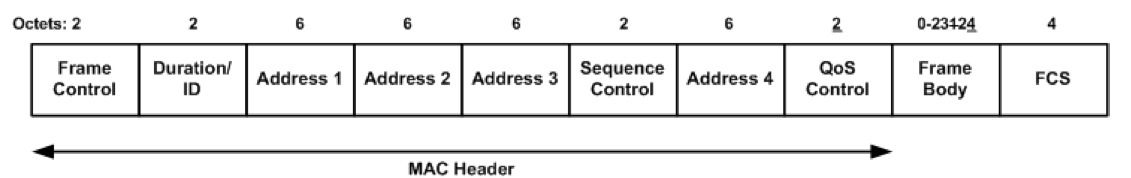
\includegraphics[angle=0, keepaspectratio=true, width=15cm]{images/mac_header2}
		\caption{MAC Frame Format}
		\label{mac_packet}
	\end{figure}
	
	The total header cost in terms of bytes is fixed to 32 bytes (octets) over a variable size of the frame body from 0 to 2304 bytes plus any overhead from security encapsulation. The frame body size is determined by the maximum MSDU + ICV + IV , where ICV (Integrity Check Value) and IV (Initialization Vector) need to WEP and MSDU is the Mac Service Data Unit. Therefore the real throughput depends by frame body length.\\
	
	To calculate the teorical throughput in the case of 802.11b we have to consider the theoretical throughput of DSSS
		
	\begin{table}[h!]
		\begin{tabularx}{15cm}{ | X | X | X | X | X | }
			\hline
				 & \multicolumn{2}{|c|}{ 802.11b (DSSS)} & \multicolumn{2}{|c|}{ 802.11g-only (OFDM)} \\
				 \hline
				 & 5.5 Mbit/s & 11 Mbit/s & 6 Mbit/s & 54 Mbit/s \\
			\hline
				DIFS & 50 ?s & 50 ?s & 28 ?s & 28 ?s \\
			\hline
				SIFS & 10 ?s & 10 ?s & 10 ?s & 10 ?s \\
			\hline
				CW & 310 ?s & 310 ?s & 139.5 ?s & 139.5 ?s \\
			\hline
				PLPC PREAMBLE + PLPC HEADER & 96 ?s & 96 ?s & 26 ?s & 26 ?s \\
			\hline
				HEADER MAC + LLC & 52.36 ?s & 26.18 ?s & 48 ?s & 5.33 ?s \\
			\hline
				HEADER IP + UDP & 40.73 ?s & 20.36 ?s & 37.33 ?s & 4.15 ?s \\
			\hline
				DATA & 2138.18 ?s & 1069.09 ?s & 1960 ?s & 217.78 \\
			\hline
				TAIL DATA & -- & -- & 1 ?s & 0.11 ?s \\
			\hline
				ACK PLPC PREAMBLE + HEADER & 96 ?s & 96 ?s & 26 ?s & 26 ?s \\
			\hline
				ACK & 20.36 ?s & 10.18 ?s & 18.67 ?s & 2.07 ?s \\
			\hline
				TAIL ACK & -- & -- & 1 ?s & 0.25 ?s \\
			\hline
			\hline
				TOTAL & 2813.63 ?s & 1687.81 & 2295.5 & 459.19 \\
			\hline
			
		\end{tabularx}
	\end{table}
	
	
	\begin{gather*}
		Throughput_{FIS\ UDP} = \\\\
		= \frac{ ( DATA_{bit} + HEADER\ IP_{bit} + HEADER\ UDP_{bit} + HEADER\ MAC_{bit} ) x 8 }{ FRAME_{seconds} } = \\\\
		= \frac{ 1532 x 8 }{  FRAME_{seconds} } \\\\
	\end{gather*}

	
% Calculate protocols upperbound limitations and similar things (report the formulas!).
% DO NOT USE PROFESSOR SLIDES AS SOURCE OF INFORMATIONS SINCE MOST OF VALUES ARE COMPLETELY WRONG!!!!!!!!!
% Download the IEEE standard from here: http://disi.unitn.it/locigno/didattica/NC/802.11-2007.pdf and make a large use of ^F.

	








